\documentclass[aspectratio=169,11pt]{beamer}

\def\courseTitle{Industrial Security (Master)}
\def\courseSubtitle{Section 05 -- Secure-by-Design Architectures}
\def\sectionNumber{05}
\def\sectionTitle{Secure-by-Design Architectures}

% =====================================================================
% Industrial Security lecture series -- modern Beamer preamble.
%
% Each slide deck must define the following BEFORE \input{}-ing this:
%   \def\courseTitle{...}        e.g. Industrial Security (Bachelor)
%   \def\courseSubtitle{...}     e.g. Section 3 -- Network Architecture
%   \def\sectionNumber{...}      e.g. 03
%   \def\sectionTitle{...}       e.g. Industrial Network Architectures
%
% Optional:
%   \def\courseAuthor{...}       defaults to "Lecture Notes"
%   \def\courseInstitute{...}    defaults to "Department of Computer Science"
%   \def\companyLogo{...}        path to a logo image (PDF/PNG/JPG).
%
% Callout macros (use anywhere inside a frame):
%   \begin{notebox}{title}      ... \end{notebox}
%   \begin{importantbox}{title} ... \end{importantbox}
%   \begin{warningbox}{title}   ... \end{warningbox}
%   \begin{tipbox}{title}       ... \end{tipbox}
%   \begin{defbox}{title}       ... \end{defbox}
%   \begin{takeawaybox}{title}  ... \end{takeawaybox}
%   \begin{quotebox}            ... \end{quotebox}
% =====================================================================

% --- Speaker-notes mode (toggled by Makefile via -usepretex) ----------
% When notesmode=1, build a side-by-side slide+notes PDF for the
% lecturer. When unset/0, build the clean slides-only PDF.
\providecommand{\notesmode}{0}
\ifnum\notesmode=1
  \usepackage{pgfpages}
  \setbeameroption{show notes on second screen=right}
  \setbeamerfont{note page}{size=\small}
\fi

\usepackage[utf8]{inputenc}
\usepackage[T1]{fontenc}
\usepackage[english]{babel}
% Modern type pair: IBM Plex Sans for text, IBM Plex Mono for code.
% Math stays in lmodern; Plex is the dominant family on every text frame.
\usepackage{plex-sans}
\usepackage{plex-mono}
\renewcommand{\familydefault}{\sfdefault}
\usepackage[activate={true,nocompatibility},final,tracking=true,kerning=true,spacing=true,factor=1100,stretch=10,shrink=10]{microtype}
\usepackage{graphicx}
\usepackage{listings}
\usepackage{xcolor}
\usepackage{colortbl}
\usepackage{tikz}
\usepackage{booktabs}
\usepackage{array}
\usepackage{hyperref}
\usepackage{amsmath}
\usepackage{amssymb}
\usepackage{tcolorbox}
\tcbuselibrary{skins, breakable, raster}
\usepackage{fontawesome5}

% =====================================================================
% Shared TikZ styles for the Industrial Security lecture series.
% Loaded by every slide deck and exercise sheet that uses TikZ.
% =====================================================================

\usetikzlibrary{
  arrows.meta,
  shapes,
  shapes.geometric,
  shapes.symbols,
  shapes.multipart,
  positioning,
  fit,
  calc,
  backgrounds,
  decorations.pathmorphing,
  decorations.pathreplacing,
  decorations.text,
  patterns,
  matrix,
  shadows
}

% --- colour palette --------------------------------------------------
\definecolor{isOT}{HTML}{1F4E79}     % OT (deep blue)
\definecolor{isIT}{HTML}{6F2DA8}     % IT (purple)
\definecolor{isSafety}{HTML}{C00000} % safety red
\definecolor{isNet}{HTML}{2E7D32}    % network green
\definecolor{isAttack}{HTML}{B23A48} % attack red
\definecolor{isAccent}{HTML}{E08E0B} % amber
\definecolor{isMute}{HTML}{6B6B6B}   % grey
\definecolor{isLight}{HTML}{EDF2F8}  % light background
\definecolor{isPLC}{HTML}{2C5282}
\definecolor{isHMI}{HTML}{2F855A}
\definecolor{isSCADA}{HTML}{6B46C1}

% --- generic node styles --------------------------------------------
\tikzset{
  isnode/.style={
    draw, rounded corners=2pt, minimum height=8mm, minimum width=18mm,
    font=\small, align=center, thick
  },
  isbox/.style={isnode, fill=isLight},
  plc/.style={isnode, fill=isPLC!15, draw=isPLC, thick},
  hmi/.style={isnode, fill=isHMI!15, draw=isHMI, thick},
  scada/.style={isnode, fill=isSCADA!15, draw=isSCADA, thick},
  sensor/.style={isnode, fill=isNet!10, draw=isNet, minimum height=6mm, minimum width=14mm, font=\scriptsize},
  actuator/.style={isnode, fill=isAccent!15, draw=isAccent, minimum height=6mm, minimum width=14mm, font=\scriptsize},
  firewall/.style={isnode, fill=isAttack!15, draw=isAttack, thick},
  server/.style={isnode, fill=isMute!15, draw=isMute!80, thick},
  switch/.style={isnode, fill=isLight, draw=black!60, minimum height=6mm, minimum width=14mm, font=\scriptsize},
  workstation/.style={isnode, fill=white, draw=isOT, thick},
  attacker/.style={isnode, fill=isAttack!20, draw=isAttack, thick, font=\small\bfseries},
  inetnode/.style={draw, ellipse, minimum width=24mm, minimum height=10mm, font=\scriptsize, fill=isLight, thick},
  process/.style={isnode, fill=isOT!15, draw=isOT, thick, minimum width=24mm},
  zone/.style={
    draw, rounded corners=4pt, thick, dashed, inner sep=4mm
  },
  conduit/.style={-{Stealth[length=2.5mm]}, thick, isNet!80!black},
  attack/.style={-{Stealth[length=2.5mm]}, thick, isAttack, dashed},
  flow/.style={-{Stealth[length=2.5mm]}, thick, isOT!70!black},
  netline/.style={thick, black!60},
  axisline/.style={-{Stealth[length=2mm]}, thick, black!70},
  tag/.style={font=\scriptsize\itshape, fill=white, inner sep=1pt},
  level/.style={
    draw, fill=isLight, minimum width=0.85\linewidth, minimum height=8mm,
    font=\small, anchor=west
  },
  brace/.style={decorate, decoration={brace, amplitude=4pt, raise=2pt}},
  legendbox/.style={draw, rounded corners=2pt, fill=isLight, inner sep=2mm, font=\scriptsize, align=left}
}

% --- handy macros ----------------------------------------------------
% \plcicon, \hmiicon etc as simple labelled boxes; useful inline.
\newcommand{\plcicon}[1][PLC]{\tikz[baseline=-0.6ex]{\node[plc, minimum width=10mm, minimum height=5mm, font=\scriptsize, inner sep=1pt]{#1};}}
\newcommand{\hmiicon}[1][HMI]{\tikz[baseline=-0.6ex]{\node[hmi, minimum width=10mm, minimum height=5mm, font=\scriptsize, inner sep=1pt]{#1};}}
\newcommand{\fwicon}[1][FW]{\tikz[baseline=-0.6ex]{\node[firewall, minimum width=10mm, minimum height=5mm, font=\scriptsize, inner sep=1pt]{#1};}}


\graphicspath{{.}{../../../template/}}

% --- defaults --------------------------------------------------------
\providecommand{\courseAuthor}{Lecture Notes}
\providecommand{\courseInstitute}{Department of Computer Science}
\providecommand{\companyLogo}{logo}

% --- modern palette --------------------------------------------------
\definecolor{slideAccent}{HTML}{1F4E79}       % primary navy
\definecolor{slideSecondary}{HTML}{E08E0B}    % amber accent

% --- Corporate branding overrides ------------------------------------
% A user-editable `branding.tex` at the repo root can override the
% logo path, author/institute lines, and brand colours. If the file is
% missing the built-in defaults above stay in effect.
\IfFileExists{../../../branding.tex}{% =====================================================================
% Corporate / institutional branding -- single file to customise the
% look of the entire course (slides, notes, exercises, labs).
%
% HOW TO REBRAND IN UNDER A MINUTE:
%   1. Replace `branding/logo.pdf` with your own logo
%      (PDF preferred; PNG and JPG also work -- name it `logo.<ext>`).
%   2. (Optional) change the two colours below to your brand palette.
%   3. (Optional) override the author/institute lines below.
%   4. Re-run `make` at the repo root. That's it.
%
% Everything in this file has sensible defaults; you can delete a line
% to fall back to the built-in defaults, or comment it out.
%
% This file is loaded automatically by the slides, exercise, and lab
% preambles -- you never need to \input it manually.
% =====================================================================

% --- Logo --------------------------------------------------------------
% Path is resolved from each leaf-build directory; the default points at
% the shared `branding/` folder at the repo root. If you put your logo
% somewhere else, set the full or relative path here (without extension):
\renewcommand{\companyLogo}{../../../branding/logo}

% --- Author / institute (appears on the title page footer) ------------
\renewcommand{\courseAuthor}{}
\renewcommand{\courseInstitute}{}

% --- Brand colours ----------------------------------------------------
% slideAccent      = primary brand colour (title bands, accent rule)
% slideSecondary   = secondary brand colour (section badge, highlight)
% Both use HTML hex codes. Keep enough contrast against white text.
\definecolor{slideAccent}{HTML}{00205B}      % deep navy
\definecolor{slideSecondary}{HTML}{00A0DC}   % light blue accent
}{}
\definecolor{slideTitle}{HTML}{0F2A44}        % near-black navy
\definecolor{slideMuted}{HTML}{6B6B6B}
\definecolor{slideBg}{HTML}{FFFFFF}
\definecolor{slidePanel}{HTML}{F4F7FB}
\definecolor{slideRule}{HTML}{D6DEE8}

% Callout colours
\definecolor{calNote}{HTML}{1F4E79}
\definecolor{calImportant}{HTML}{B23A48}
\definecolor{calWarning}{HTML}{C77700}
\definecolor{calTip}{HTML}{2E7D32}
\definecolor{calDef}{HTML}{6B46C1}
\definecolor{calTake}{HTML}{0F2A44}

% --- beamer theme ---------------------------------------------------
\useinnertheme{rectangles}
\usefonttheme{professionalfonts}

\setbeamertemplate{navigation symbols}{}
\setbeamertemplate{itemize items}[circle]
\setbeamertemplate{enumerate items}[default]
\setbeamertemplate{section in toc}[ball numbered]
\setbeamercolor{section in toc}{fg=slideTitle}

% Colours
\setbeamercolor{normal text}{fg=slideTitle, bg=slideBg}
\setbeamercolor{title}{fg=slideAccent}
\setbeamercolor{subtitle}{fg=slideMuted}
\setbeamercolor{frametitle}{fg=slideAccent}
\setbeamercolor{structure}{fg=slideAccent}
\setbeamercolor{itemize item}{fg=slideAccent}
\setbeamercolor{itemize subitem}{fg=slideSecondary}
\setbeamercolor{block title}{fg=white, bg=slideAccent}
\setbeamercolor{block body}{fg=slideTitle, bg=slidePanel}
\setbeamercolor{alerted text}{fg=slideSecondary}

% Fonts
\setbeamerfont{title}{series=\bfseries, size=\Large}
\setbeamerfont{subtitle}{series=\mdseries, size=\normalsize}
\setbeamerfont{frametitle}{series=\bfseries, size=\large}
\setbeamerfont{block title}{series=\bfseries, size=\normalsize}
\setbeamerfont{footline}{size=\tiny}

% --- frametitle: title bar + accent underline + section badge -------
% The accent rules are wrapped in a zero-width box so they never
% contribute to the surrounding hbox width (no Overfull warnings).
\setbeamertemplate{frametitle}{%
  \nointerlineskip
  \begin{beamercolorbox}[wd=\paperwidth, ht=2.8ex, dp=1.6ex, leftskip=1.2em, rightskip=1.2em]{frametitle}%
    \usebeamerfont{frametitle}\insertframetitle%
    \hfill
    {\color{slideMuted}\small \sectionNumber}%
  \end{beamercolorbox}%
  \nointerlineskip
  \makebox[0pt][l]{\hspace*{1.2em}\textcolor{slideSecondary}{\rule{2.5em}{1pt}}\textcolor{slideAccent}{\rule{\dimexpr\paperwidth-3.7em\relax}{1pt}}}%
  \par\vskip4pt
}

% --- footer ---------------------------------------------------------
\defbeamertemplate*{footline}{is-footer}{%
  \leavevmode%
  \hbox{%
    \begin{beamercolorbox}[wd=.55\paperwidth, ht=2.4ex, dp=1ex, leftskip=1em]{author in head/foot}%
      {\color{slideMuted}\tiny \courseTitle{} \;\; $\bullet$ \;\; Section \sectionNumber{} -- \sectionTitle}%
    \end{beamercolorbox}%
    \begin{beamercolorbox}[wd=.45\paperwidth, ht=2.4ex, dp=1ex, rightskip=1em]{title in head/foot}%
      \hfill {\color{slideMuted}\tiny \insertframenumber{} / \inserttotalframenumber}%
    \end{beamercolorbox}%
  }%
  \vskip2pt
}

% --- listings -------------------------------------------------------
\definecolor{codebg}{HTML}{F4F7FB}
\definecolor{codekw}{HTML}{0F2A44}
\definecolor{codestr}{HTML}{8B3A3A}
\definecolor{codecom}{HTML}{5A7D54}

\lstset{
    backgroundcolor=\color{codebg},
    basicstyle=\ttfamily\scriptsize\color{slideTitle},
    keywordstyle=\color{codekw}\bfseries,
    stringstyle=\color{codestr},
    commentstyle=\color{codecom}\itshape,
    breaklines=true,
    frame=leftline,
    framerule=2pt,
    rulecolor=\color{slideAccent},
    numbers=left,
    numberstyle=\tiny\color{slideMuted},
    numbersep=8pt,
    showstringspaces=false,
    tabsize=2,
    captionpos=b,
    xleftmargin=0.6em
}

% --- callout boxes --------------------------------------------------
% Shared base style for all callout boxes.
% Subtle drop shadow gives the boxes a hint of elevation without distraction.
\tcbset{
  isCallout/.style={
    enhanced, breakable, sharp corners=northeast,
    arc=2pt, boxrule=0pt,
    leftrule=3pt,
    fonttitle=\bfseries\small,
    coltitle=white,
    fontupper=\small,
    left=2mm, right=2mm, top=1.5mm, bottom=1.5mm,
    drop fuzzy shadow=black!30,
    title={#1}
  }
}

\newtcolorbox{notebox}[1]{
  isCallout={#1},
  colback=calNote!8, colframe=calNote, leftrule=3pt,
  colbacktitle=calNote, attach boxed title to top left={xshift=2mm, yshift=-1.2mm},
  boxed title style={colback=calNote, arc=1pt, boxrule=0pt, left=2mm, right=2mm, top=0.5mm, bottom=0.5mm}
}

\newtcolorbox{importantbox}[1]{
  isCallout={#1},
  colback=calImportant!7, colframe=calImportant, leftrule=4pt,
  colbacktitle=calImportant, attach boxed title to top left={xshift=2mm, yshift=-1.2mm},
  boxed title style={colback=calImportant, arc=1pt, boxrule=0pt, left=2mm, right=2mm, top=0.5mm, bottom=0.5mm}
}

\newtcolorbox{warningbox}[1]{
  isCallout={#1},
  colback=calWarning!10, colframe=calWarning, leftrule=4pt,
  colbacktitle=calWarning, attach boxed title to top left={xshift=2mm, yshift=-1.2mm},
  boxed title style={colback=calWarning, arc=1pt, boxrule=0pt, left=2mm, right=2mm, top=0.5mm, bottom=0.5mm}
}

% Alias warnbox = warningbox, with an optional title (default = "Caution")
\newtcolorbox{warnbox}[1][Caution]{
  isCallout={#1},
  colback=calWarning!10, colframe=calWarning, leftrule=4pt,
  colbacktitle=calWarning, attach boxed title to top left={xshift=2mm, yshift=-1.2mm},
  boxed title style={colback=calWarning, arc=1pt, boxrule=0pt, left=2mm, right=2mm, top=0.5mm, bottom=0.5mm}
}

\newtcolorbox{tipbox}[1]{
  isCallout={#1},
  colback=calTip!8, colframe=calTip, leftrule=3pt,
  colbacktitle=calTip, attach boxed title to top left={xshift=2mm, yshift=-1.2mm},
  boxed title style={colback=calTip, arc=1pt, boxrule=0pt, left=2mm, right=2mm, top=0.5mm, bottom=0.5mm}
}

\newtcolorbox{defbox}[1]{
  isCallout={#1},
  colback=calDef!8, colframe=calDef, leftrule=3pt,
  colbacktitle=calDef, attach boxed title to top left={xshift=2mm, yshift=-1.2mm},
  boxed title style={colback=calDef, arc=1pt, boxrule=0pt, left=2mm, right=2mm, top=0.5mm, bottom=0.5mm}
}

\newtcolorbox{takeawaybox}[1]{
  enhanced, breakable, arc=3pt, boxrule=0pt,
  colback=calTake!7, colframe=calTake,
  toptitle=2mm, bottomtitle=2mm,
  fonttitle=\bfseries\normalsize, coltitle=white,
  colbacktitle=calTake,
  fontupper=\small,
  title={\faStar~Key Takeaway: #1},
  left=3mm, right=3mm, top=2mm, bottom=2mm
}

\newtcolorbox{quotebox}{
  enhanced, breakable, arc=2pt, boxrule=0pt,
  colback=slidePanel, colframe=slideMuted,
  leftrule=3pt, top=2mm, bottom=2mm, left=3mm, right=3mm,
  fontupper=\itshape\small,
}

% Convenience: inline highlight badge
\newcommand{\remembertag}{\tikz[baseline=-0.7ex]\node[fill=calImportant, text=white, font=\scriptsize\bfseries, rounded corners=2pt, inner sep=2pt]{REMEMBER};}
\newcommand{\tldr}{\tikz[baseline=-0.7ex]\node[fill=calTake, text=white, font=\scriptsize\bfseries, rounded corners=2pt, inner sep=2pt]{TL;DR};}

% Source attribution: tiny grey line, anchored bottom-left of the content area
% Usage:  \source{Symantec, \emph{W32.Stuxnet Dossier} v1.4, 2011.}
% Multiple sources:  \source{X.\ Y., 2018; Z, 2020.}
\newcommand{\source}[1]{%
  \par\nointerlineskip\vspace{0.4mm}%
  {\color{slideMuted}\fontsize{5.5}{6.5}\selectfont\textit{Source:} #1\par}%
}

% References slide: aggregate citations + further reading at the end of a section.
% Usage:  \referencesframe{ \item ... \item ... }
% The `frame` environment must be written literally in the deck, so this is a
% macro rather than a wrapper environment (beamer collects the frame body and
% trips over \newenvironment wrappers).
%
% allowframebreakstemplate=\insertcontinuationcount silences the trailing roman
% numeral when content fits on a single page.
\setbeamertemplate{frametitle continuation}[from second]
\newcommand{\referencesframe}[1]{%
  \begin{frame}[allowframebreaks]{References -- Section \sectionNumber}
    \fontsize{7.5}{9}\selectfont
    \setlength{\itemsep}{1pt}
    \begin{itemize}#1\end{itemize}
  \end{frame}%
}

% --- title page -----------------------------------------------------
\title[\courseTitle]{\courseTitle}
\subtitle{\courseSubtitle}
\author{\courseAuthor}
\institute{\courseInstitute}
\date{}

% Logo lookup: try the section directory, then the shared template/.
\newcommand{\showlogo}[1][2cm]{%
  \IfFileExists{\companyLogo.pdf}{\includegraphics[width=#1]{\companyLogo}}{%
    \IfFileExists{\companyLogo.png}{\includegraphics[width=#1]{\companyLogo}}{%
      \IfFileExists{\companyLogo.jpg}{\includegraphics[width=#1]{\companyLogo}}{%
        \IfFileExists{../../../template/\companyLogo.pdf}{\includegraphics[width=#1]{../../../template/\companyLogo}}{%
          \rule{0pt}{0pt}}}}}}

\setbeamertemplate{title page}{%
  \begin{tikzpicture}[remember picture, overlay]
    % accent band (taller to fit wrapped titles)
    \fill[slideAccent] (current page.north west) rectangle ([yshift=-3.4cm]current page.north east);
    \fill[slideSecondary] ([yshift=-3.4cm]current page.north west) rectangle ([yshift=-3.55cm]current page.north east);
    % section badge
    \node[fill=slideSecondary, text=white, font=\bfseries\normalsize, rounded corners=3pt, inner sep=4pt, anchor=north west]
      at ([xshift=1.2cm, yshift=-0.7cm]current page.north west) {Section \sectionNumber};
    % Course title (wraps if long)
    \node[anchor=north west, text=white, font=\bfseries\Large, align=left, text width=11cm]
      at ([xshift=1.2cm, yshift=-1.5cm]current page.north west) {\courseTitle};
    % Subtitle (wraps; smaller, separated)
    \node[anchor=north west, text=white, font=\mdseries\small, align=left, text width=11cm]
      at ([xshift=1.2cm, yshift=-2.7cm]current page.north west) {\courseSubtitle};
    \node[anchor=north east] at ([xshift=-1.2cm, yshift=-1.0cm]current page.north east)
      {\showlogo[2cm]};
    \node[anchor=south west, text=slideMuted, font=\small, align=left, text width=11cm]
      at ([xshift=1.2cm, yshift=1.0cm]current page.south west)
      {\textbf{\sectionTitle}\\[2pt]\textit{\courseAuthor}\\{\scriptsize\courseInstitute}};
  \end{tikzpicture}
}

% --- helper macros --------------------------------------------------
\newcommand{\learningobjectives}[1]{%
  \begin{frame}{Learning Objectives}
    \begin{tipbox}{\faGraduationCap~By the end of this section you will be able to}
      \begin{itemize}\setlength{\itemsep}{2pt}#1\end{itemize}
    \end{tipbox}
  \end{frame}}

\newcommand{\sectionoverviewframe}{%
  \begin{frame}[plain,noframenumbering]
    \titlepage
  \end{frame}
  \begin{frame}{Outline -- Section \sectionNumber}
    \tableofcontents
  \end{frame}}

\AtBeginSection[]{%
  \begin{frame}[plain,noframenumbering]
    \begin{tikzpicture}[remember picture, overlay]
      \fill[slideAccent] (current page.north west) rectangle (current page.south east);
      \fill[slideSecondary] ([yshift=-1pt]current page.center -| current page.west)
                            rectangle ([yshift=1pt]current page.center -| current page.east);
      \node[text=white, font=\scriptsize, anchor=south west]
        at ([xshift=1.2cm, yshift=1.0cm]current page.south west)
        {Section \sectionNumber{} -- \sectionTitle};
      \node[text=slideSecondary, font=\bfseries\Huge, anchor=south]
        at ([yshift=0.4cm]current page.center)
        {\thesection};
      \node[text=white, font=\bfseries\LARGE, align=center, anchor=north, text width=12cm]
        at ([yshift=-0.6cm]current page.center)
        {\insertsection};
    \end{tikzpicture}
  \end{frame}}

\newcommand{\closingframe}{%
  \begin{frame}[plain,noframenumbering]
    \begin{tikzpicture}[remember picture, overlay]
      \fill[slideAccent] (current page.north west) rectangle (current page.south east);
      \node[text=white, font=\bfseries\Huge, anchor=center, align=center, text width=14cm]
        at ([yshift=8mm]current page.center) {End of Section \sectionNumber};
      \fill[slideSecondary] ([xshift=-1.5cm, yshift=-4mm]current page.center)
                            rectangle ([xshift=1.5cm, yshift=-6mm]current page.center);
      \node[text=white, font=\large, anchor=north, align=center, text width=14cm]
        at ([yshift=-1.2cm]current page.center) {\sectionTitle};
      \node[text=slideSecondary, font=\normalsize, anchor=south] at ([yshift=1.2cm]current page.south) {Questions and discussion};
      \node[anchor=south east] at ([xshift=-1cm, yshift=1cm]current page.south east) {\showlogo[1.5cm]};
    \end{tikzpicture}
  \end{frame}}


\begin{document}

\sectionoverviewframe

\learningobjectives{
  \item Translate security requirements into early-design decisions on a greenfield plant.
  \item Apply IEC 62443 zones, conduits and target SLs from the FEED phase.
  \item Choose vendor-agnostic patterns: data diodes, brokered access, immutable backups.
  \item Make security trade-offs explicit and defensible to operators and finance.
  \item Build the contractual artefacts (vendor SDL, SBOM, ATPs) that survive procurement.
}

\section{Why Design First}

\begin{frame}{Bolt-on vs.\ Built-in}
\centering
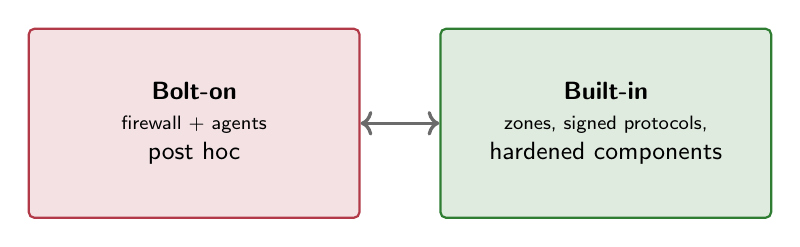
\begin{tikzpicture}[node distance=10mm]
  \node[isbox, fill=isAttack!15, draw=isAttack, minimum width=42mm, minimum height=24mm, align=center, font=\small] (b) {\textbf{Bolt-on}\\\scriptsize firewall + agents\\post hoc};
  \node[isbox, fill=isNet!15, draw=isNet, minimum width=42mm, minimum height=24mm, align=center, font=\small, right=of b] (i) {\textbf{Built-in}\\\scriptsize zones, signed protocols,\\hardened components};
  \draw[<->, very thick, isMute] (b) -- (i);
\end{tikzpicture}
\vspace{2mm}
\begin{importantbox}{Cost curve}
Security retrofits in OT typically cost 5--10$\times$ a design-phase decision and take a planned outage. Built-in choices avoid both.
\end{importantbox}
\source{INL CCE programme, multiple case studies 2018--2022.}
\end{frame}

\begin{frame}{The Greenfield Window}
\centering
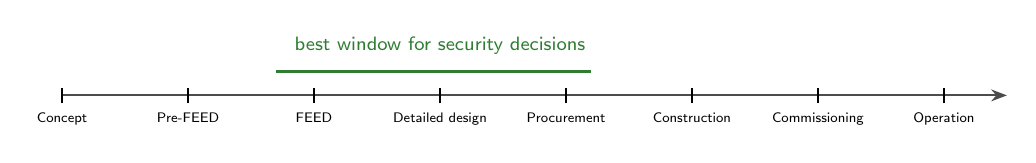
\begin{tikzpicture}[x=1.6cm]
  \draw[axisline] (0,0) -- (7.5,0);
  \foreach \x/\name in {0/{Concept},1/{Pre-FEED},2/{FEED},3/{Detailed design},4/{Procurement},5/{Construction},6/{Commissioning},7/{Operation}}{
    \draw[thick] (\x,-1mm) -- (\x,1mm);
    \node[font=\tiny, below=1mm] at (\x,0) {\name};
  }
  \draw[very thick, isNet] (1.7,3mm) -- (4.2,3mm);
  \node[font=\scriptsize, isNet, above=1mm] at (3,3mm) {best window for security decisions};
\end{tikzpicture}
\vspace{1mm}
\begin{notebox}{FEED phase}
Front-End Engineering Design is when zones, conduits, SLs become contractually binding. Earlier = cheaper; later = compromised.
\end{notebox}
\end{frame}

\section{Pattern Library}

\begin{frame}{Pattern 1 -- Strict Purdue with Diodes}
\centering
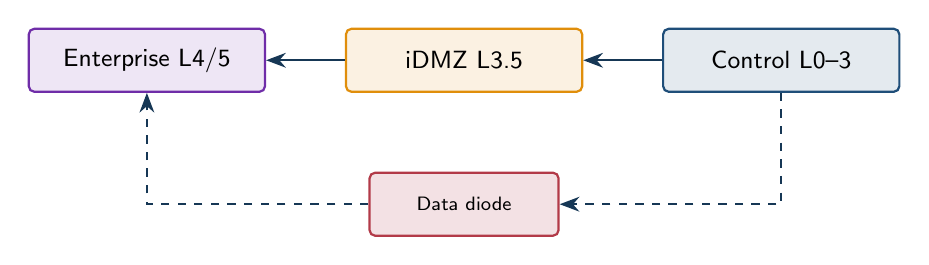
\begin{tikzpicture}[node distance=10mm]
  \node[isbox, fill=isIT!12, draw=isIT, minimum width=30mm] (it) {Enterprise L4/5};
  \node[isbox, fill=isAccent!12, draw=isAccent, right=of it, minimum width=30mm] (dmz) {iDMZ L3.5};
  \node[isbox, fill=isOT!12, draw=isOT, right=of dmz, minimum width=30mm] (ot) {Control L0--3};
  \node[firewall, below=of dmz, minimum width=24mm, font=\scriptsize] (d) {Data diode};
  \draw[flow] (ot) -- (dmz); \draw[flow] (dmz) -- (it);
  \draw[flow, dashed] (ot.south) |- (d.east);
  \draw[flow, dashed] (d.west) -| (it.south);
\end{tikzpicture}
\vspace{2mm}
\begin{notebox}{When it earns its cost}
SIS-adjacent zones; export of safety telemetry to the corporate side; regulatory reporting feeds.
\end{notebox}
\end{frame}

\begin{frame}{Pattern 2 -- Hub-and-Spoke iDMZ}
\centering
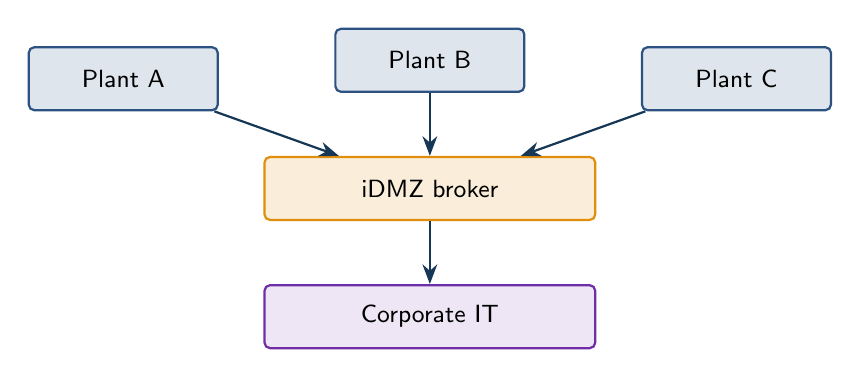
\begin{tikzpicture}[node distance=8mm]
  \node[isbox, fill=isAccent!15, draw=isAccent, minimum width=42mm, font=\small] (idmz) {iDMZ broker};
  \node[plc, above left=of idmz, minimum width=24mm] (plc1) {Plant A};
  \node[plc, above=of idmz, minimum width=24mm] (plc2) {Plant B};
  \node[plc, above right=of idmz, minimum width=24mm] (plc3) {Plant C};
  \node[isbox, fill=isIT!12, draw=isIT, below=of idmz, minimum width=42mm, font=\small] (it) {Corporate IT};
  \foreach \n in {plc1,plc2,plc3}{\draw[flow] (\n) -- (idmz);}
  \draw[flow] (idmz) -- (it);
\end{tikzpicture}
\vspace{2mm}
\begin{notebox}{Multi-site benefit}
Single point of policy enforcement for vendor remote access, historian replication, software updates -- across all plants.
\end{notebox}
\end{frame}

\begin{frame}{Pattern 3 -- Identity Brokered Remote Access}
\centering
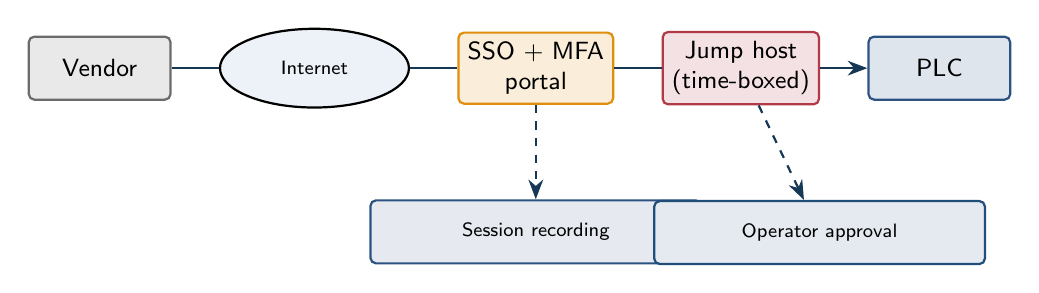
\begin{tikzpicture}[node distance=6mm]
  \node[isbox, fill=isMute!15, draw=isMute] (vend) {Vendor};
  \node[inetnode, fill=isLight, right=of vend] (inet) {Internet};
  \node[isbox, fill=isAccent!15, draw=isAccent, right=of inet, font=\small, align=center] (broker) {SSO + MFA\\portal};
  \node[isbox, fill=isAttack!15, draw=isAttack, right=of broker, font=\small, align=center] (jump) {Jump host\\(time-boxed)};
  \node[plc, right=of jump] (plc) {PLC};
  \node[isbox, fill=isPLC!12, draw=isPLC, below=12mm of broker, font=\scriptsize, minimum width=42mm] (rec) {Session recording};
  \node[isbox, fill=isOT!12, draw=isOT, below=12mm of jump, font=\scriptsize, minimum width=42mm, xshift=10mm] (op) {Operator approval};
  \draw[flow] (vend) -- (inet) -- (broker) -- (jump) -- (plc);
  \draw[flow, dashed] (broker) -- (rec);
  \draw[flow, dashed] (jump) -- (op);
\end{tikzpicture}
\source{Cyolo / Claroty xDome Secure Access / Dispel design patterns, 2020--2024.}
\end{frame}

\begin{frame}{Pattern 4 -- Crypto-Agile Protocol Stack}
\centering
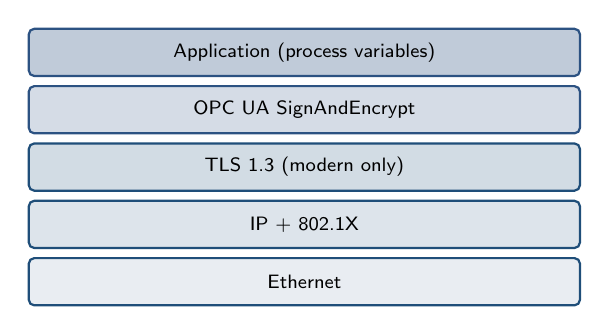
\begin{tikzpicture}[node distance=1mm]
  \node[isbox, fill=isOT!10, draw=isOT, minimum width=70mm, minimum height=6mm, font=\scriptsize] (eth) {Ethernet};
  \node[isbox, fill=isOT!15, draw=isOT, minimum width=70mm, minimum height=6mm, font=\scriptsize, above=of eth] (ip) {IP + 802.1X};
  \node[isbox, fill=isOT!20, draw=isOT, minimum width=70mm, minimum height=6mm, font=\scriptsize, above=of ip] (tls) {TLS 1.3 (modern only)};
  \node[isbox, fill=isPLC!20, draw=isPLC, minimum width=70mm, minimum height=6mm, font=\scriptsize, above=of tls] (ua) {OPC UA SignAndEncrypt};
  \node[isbox, fill=isPLC!30, draw=isPLC, minimum width=70mm, minimum height=6mm, font=\scriptsize, above=of ua] (app) {Application (process variables)};
\end{tikzpicture}
\vspace{2mm}
\begin{notebox}{Future-proofing}
Specify in procurement: TLS 1.3+, modern cipher suites, support for cert rotation, and an explicit upgrade-path commitment from the vendor.
\end{notebox}
\end{frame}

\begin{frame}{Pattern 5 -- Immutable Backup Triad}
\centering
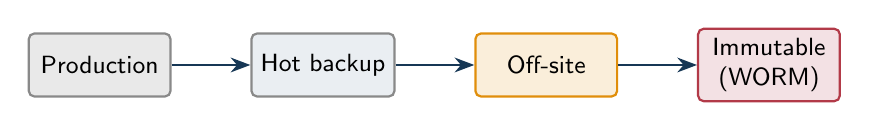
\begin{tikzpicture}[node distance=10mm]
  \node[server] (prod) {Production};
  \node[server, fill=isPLC!10, right=of prod] (b1) {Hot backup};
  \node[server, fill=isAccent!15, draw=isAccent, right=of b1] (b2) {Off-site};
  \node[server, fill=isAttack!15, draw=isAttack, right=of b2, font=\small, align=center] (b3) {Immutable\\(WORM)};
  \draw[flow] (prod) -- (b1); \draw[flow] (b1) -- (b2); \draw[flow] (b2) -- (b3);
\end{tikzpicture}
\vspace{2mm}
\begin{importantbox}{Test restore quarterly}
Backups that have never been restored are not backups.
\end{importantbox}
\end{frame}

\section{Procurement \& Contracts}

\begin{frame}{Vendor SDL Requirements}
\begin{itemize}
  \item Conformance to IEC 62443-4-1 (Secure Development Lifecycle).
  \item SBOM in CycloneDX or SPDX delivered with every release.
  \item Threat modelling for the product, reviewed every major release.
  \item Vulnerability handling per ISO/IEC 30111 with SLA on disclosure.
  \item Long-term support commitment (e.g.\ 10 years from delivery).
\end{itemize}
\begin{tipbox}{Contractual leverage}
Bake these into the purchase order. Vendors that cannot deliver an SBOM today should not be on a 20-year capital-investment list.
\end{tipbox}
\source{IEC 62443-4-1:2018 \textbar{} ISO/IEC 30111:2019 \textbar{} OWASP CycloneDX, SPDX.}
\end{frame}

\begin{frame}{Acceptance Test Procedures (ATP)}
\centering
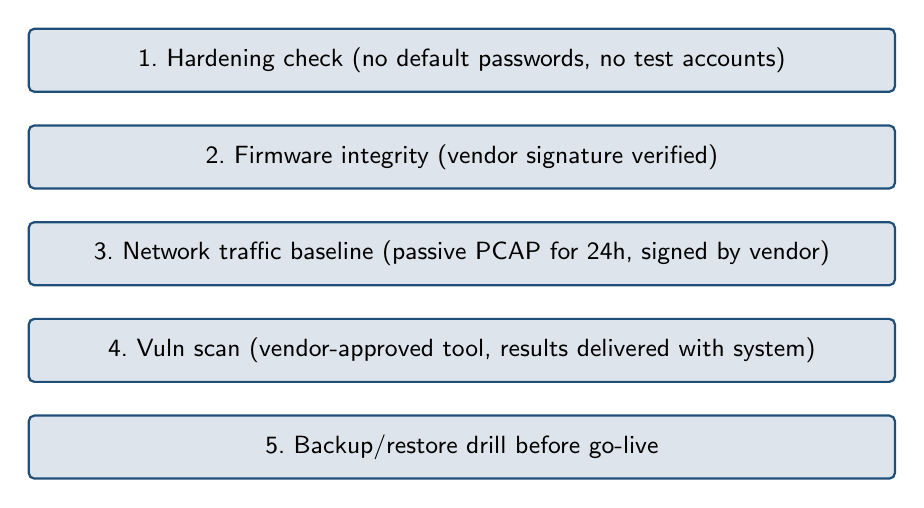
\begin{tikzpicture}[node distance=4mm]
  \node[isbox, fill=isOT!15, draw=isOT, minimum width=110mm, font=\small] (a) {1.\ Hardening check (no default passwords, no test accounts)};
  \node[isbox, fill=isOT!15, draw=isOT, minimum width=110mm, font=\small, below=of a] (b) {2.\ Firmware integrity (vendor signature verified)};
  \node[isbox, fill=isOT!15, draw=isOT, minimum width=110mm, font=\small, below=of b] (c) {3.\ Network traffic baseline (passive PCAP for 24h, signed by vendor)};
  \node[isbox, fill=isOT!15, draw=isOT, minimum width=110mm, font=\small, below=of c] (d) {4.\ Vuln scan (vendor-approved tool, results delivered with system)};
  \node[isbox, fill=isOT!15, draw=isOT, minimum width=110mm, font=\small, below=of d] (e) {5.\ Backup/restore drill before go-live};
\end{tikzpicture}
\end{frame}

\section{Trade-offs}

\begin{frame}{Where Security Trades Against Operations}
\centering
\renewcommand{\arraystretch}{1.3}
\footnotesize
\begin{tabular}{|p{3.6cm}|p{4.2cm}|p{4.2cm}|}
\hline
\rowcolor{slidePanel}
\textbf{Decision} & \textbf{Security win} & \textbf{Operational cost} \\
\hline
SignAndEncrypt OPC UA  & integrity, confidentiality   & cert lifecycle, vendor support \\
Strict iDMZ            & blast-radius limit            & multi-hop for engineers \\
MFA on jump host       & credential theft mitigated   & operator interruption \\
Application allow-list & malware execution blocked    & change control overhead \\
Data diode             & one-way egress only           & no remote control at all \\
\hline
\end{tabular}
\end{frame}

\begin{frame}{Risk Acceptance Conversation}
\begin{itemize}
  \item Frame as: ``If we do X, residual risk is Y, cost is Z.''
  \item Pair every accepted residual with a review date.
  \item Capture in a register countersigned by safety + operations + executive.
  \item Re-open whenever the threat picture changes (new APT advisory, new sector incident).
\end{itemize}
\begin{warnbox}
``We accept the risk'' without paper is no acceptance at all. Auditors and post-incident lawyers both want the paper.
\end{warnbox}
\end{frame}

\section{Migration from Brownfield}

\begin{frame}{Brownfield Reality Check}
\centering
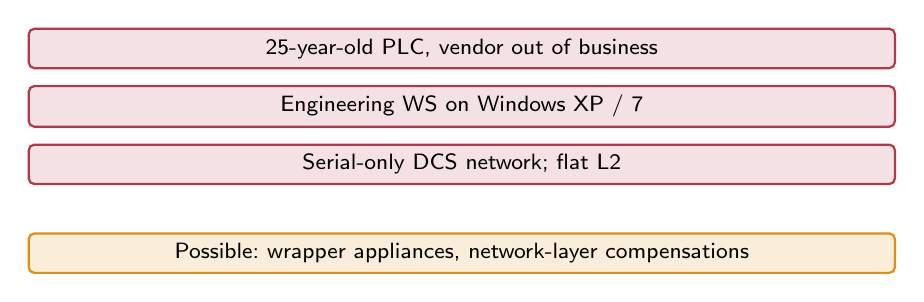
\begin{tikzpicture}[node distance=2mm]
  \node[isbox, fill=isAttack!15, draw=isAttack, minimum width=110mm, font=\footnotesize, minimum height=5mm] (a) {25-year-old PLC, vendor out of business};
  \node[isbox, fill=isAttack!15, draw=isAttack, minimum width=110mm, font=\footnotesize, minimum height=5mm, below=of a] (b) {Engineering WS on Windows XP / 7};
  \node[isbox, fill=isAttack!15, draw=isAttack, minimum width=110mm, font=\footnotesize, minimum height=5mm, below=of b] (c) {Serial-only DCS network; flat L2};
  \node[isbox, fill=isAccent!15, draw=isAccent, minimum width=110mm, font=\footnotesize, minimum height=5mm, below=6mm of c] (d) {Possible: wrapper appliances, network-layer compensations};
\end{tikzpicture}
\vspace{1mm}
\begin{notebox}{Realistic horizon}
Most secure-by-design wins arrive in the next capital project. Brownfield gets compensating controls and a roadmap.
\end{notebox}
\end{frame}

\begin{frame}{Migration Roadmap (sketch)}
\centering
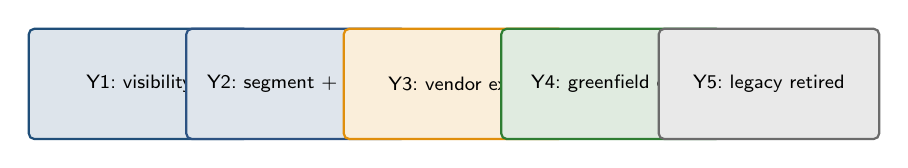
\begin{tikzpicture}[x=2.0cm]
  \foreach \i/\name/\col in {
    0/{Y1: visibility}/isOT,
    1/{Y2: segment + MFA}/isPLC,
    2/{Y3: vendor exit}/isAccent,
    3/{Y4: greenfield core}/isNet,
    4/{Y5: legacy retired}/isMute}{
    \node[isbox, fill=\col!15, draw=\col, font=\scriptsize, align=center, minimum width=28mm, minimum height=14mm]
      at (\i,0) {\name};
  }
\end{tikzpicture}
\vspace{2mm}
\begin{tipbox}{Sequence matters}
You cannot segment what you have not inventoried. You cannot retire what you have not replaced.
\end{tipbox}
\end{frame}

\begin{frame}{Summary -- Section \sectionNumber}
\begin{takeawaybox}{Build it in, not on}
\begin{itemize}\setlength{\itemsep}{2pt}
  \item Security decisions are cheapest in the FEED phase, most expensive after commissioning.
  \item A small library of patterns (Purdue+diode, iDMZ broker, brokered access, crypto-agile stack, immutable backup) covers most greenfield plants.
  \item Contractual artefacts (SDL, SBOM, ATPs) are the only thing that survives the procurement firewall.
  \item Trade-offs are unavoidable -- write them down, name an owner, set a review date.
  \item Brownfield gets compensating controls and a sequenced migration roadmap.
\end{itemize}
\end{takeawaybox}
\end{frame}

\referencesframe{
  \item IEC 62443-2-1:2010 + Amd.\,2019. \emph{IACS asset owner programme}.
  \item IEC 62443-3-2:2020. \emph{Security risk assessment for system design}.
  \item IEC 62443-3-3:2013. \emph{System security requirements and security levels}.
  \item IEC 62443-4-1:2018. \emph{Secure product development lifecycle (SDL)}.
  \item IEC 62443-4-2:2019. \emph{Technical security requirements for IACS components}.
  \item INL. \emph{Consequence-Driven Cyber-Informed Engineering (CCE)}, Bochman \& Freeman, 2021.
  \item NIST SP 800-160 Vol.\,1 Rev.\,1. \emph{Engineering Trustworthy Secure Systems}, 2022.
  \item ENISA. \emph{Good practices for IACS}, 2020 onwards.
  \item OWASP. \emph{CycloneDX Specification} for SBOMs.
  \item SPDX. \emph{Software Package Data Exchange}.
  \item Owl Cyber Defense, Waterfall Security: data-diode product literature for typical patterns.
  \item Cyolo / Dispel / Claroty xDome Secure Access: brokered remote-access design notes.
}

\closingframe

\end{document}
